\documentclass[journal]{IEEEtran}
% SPS manuscript rule: 10-point, double-column, single-spaced, margins of at least 1 inch on all sides
\usepackage[letterpaper,margin=1in]{geometry}
\usepackage{cite}
\usepackage{amsmath,amssymb,amsfonts}
\usepackage{graphicx}
\usepackage{booktabs}
\usepackage{multirow}
\usepackage{xcolor}
\usepackage{algorithm}
\usepackage{algpseudocode}
\usepackage{xr}
\externaldocument[M-]{paper}
\newcommand{\ffpp}{FF\texttt{++}}
\renewcommand{\thesection}{S\arabic{section}}
\renewcommand{\topfraction}{0.9}
\renewcommand{\dbltopfraction}{0.9}
\renewcommand{\textfraction}{0.07}
\renewcommand{\floatpagefraction}{0.85}
\renewcommand{\dblfloatpagefraction}{0.85}
\setcounter{topnumber}{3}
\setcounter{dbltopnumber}{2}
\setlength{\textfloatsep}{8pt plus 2pt minus 2pt}
% figures, tables and equations continue the numbering of the main paper (SPS supplemental-material rule)
\setcounter{figure}{4}
\setcounter{table}{8}
\setcounter{algorithm}{2}
\setcounter{equation}{6}
\begin{document}
\title{Supplementary Material for\\ Protecting Generalization in Continually Updated Deepfake Detectors}
\author{Naren~Medarametla, Ramineni~Durga~Sai~Sumanth, and~Kowsigan~M}
\markboth{Supplementary material}{Medarametla \MakeLowercase{\textit{et al.}}: Protecting Generalization in Continually Updated Deepfake Detectors}
\maketitle

This document collects development results and secondary analyses that are summarized in the main paper. Figures, tables and equations are numbered consecutively with the main paper; section numbers with the prefix S refer to this document. All numbers are produced by the released analysis scripts.

\section{Development comparison}
Development used the released GenD checkpoint, the development splits and three seeds (main paper, Section~\ref{M-sec:setup}). Table~\ref{tab:dev} and Fig.~\ref{fig:dev} report the comparison that selected the configuration later confirmed on sealed data.

\begin{table}[t]
\caption{Development results (released GenD, development splits with 8 frames per video, three seeds). FSh: FaceShifter probe AUROC after all updates, mean and [min, max] over seeds.}
\label{tab:dev}
\centering
\footnotesize
\setlength{\tabcolsep}{2.6pt}
\resizebox{\columnwidth}{!}{%
\begin{tabular}{@{}lcccccc@{}}
\toprule
Method & FSh & AA & AF & Gain & ACC$_{\mathrm{FF}}$ \\
\midrule
No update & 84.85 & 97.20 & \textendash & \textendash & 95.0 \\
Seq.\ FT & 77.06 [76.44, 77.39] & 97.78 & 0.79 & 2.10 & 79.9 \\
EWC~\cite{kirkpatrick2017ewc} & 76.67 [75.52, 77.34] & 97.73 & 0.84 & 2.10 & 79.7 \\
SDC replay~\cite{yu2020sdc} & 76.94 [75.66, 78.65] & 97.70 & 0.86 & 2.05 & 78.9 \\
Symmetric KD & 78.66 [77.57, 79.48] & 98.18 & 0.31 & 1.51 & 85.1 \\
LN merging & 80.38 [79.94, 81.01] & 97.57 & 0.30 & 0.85 & 88.1 \\
LwF~\cite{li2018lwf} & 80.49 [80.23, 80.69] & 97.95 & 0.30 & 1.39 & 86.3 \\
GA + memory & 80.69 [79.54, 81.58] & 98.42 & 0.13 & 1.38 & 87.6 \\
GA & 80.67 [79.30, 81.63] & 98.42 & 0.13 & 1.40 & 87.8 \\
GA + mem.\ + LwF & 82.84 [81.99, 83.38] & 98.26 & $-$0.01 & 1.05 & 91.1 \\
GA+LwF & \textbf{82.85} [82.05, 83.52] & 98.26 & 0.01 & 1.05 & \textbf{91.5} \\
\bottomrule
\end{tabular}%
}
\end{table}

\begin{figure}[t]
\centering
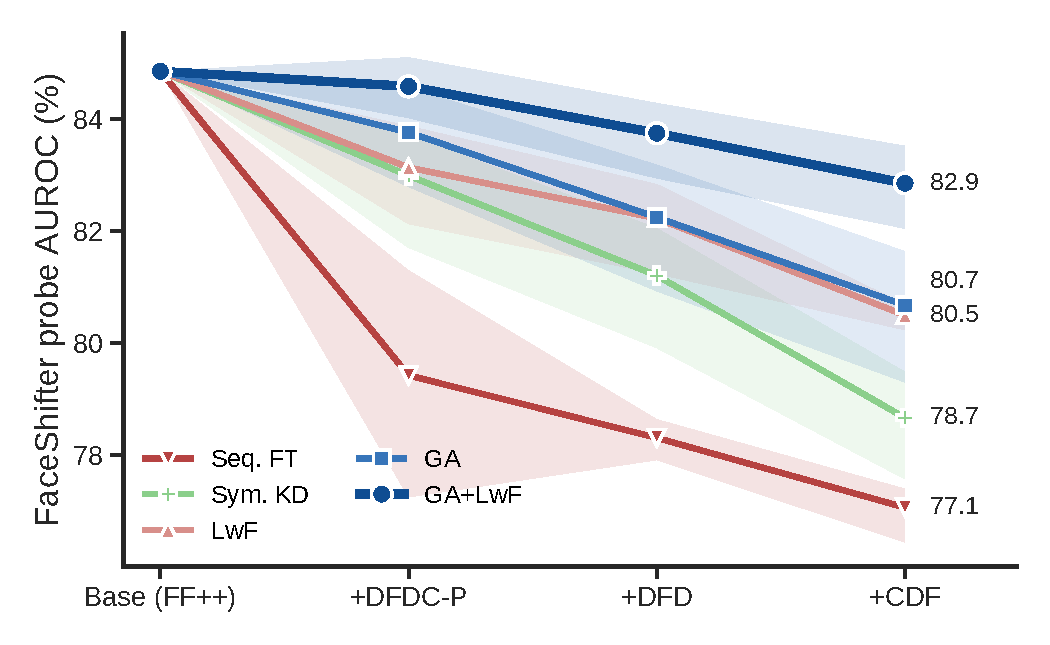
\includegraphics[width=\columnwidth]{figures/fig_dev_curves.pdf}
\caption{FaceShifter probe AUROC across the update stream on development data. Lines show the mean and shaded bands the range over three seeds.}
\label{fig:dev}
\end{figure}

\section{Where generalization is lost}
Fig.~\ref{fig:unseen} breaks the unseen-panel score down by dataset and generator for the seed-0 models of stream S1, Fig.~\ref{fig:stagewise} follows it along the three updates of S1, and Fig.~\ref{fig:shots} varies the number of videos per class and task.

\begin{figure}[t]
\centering
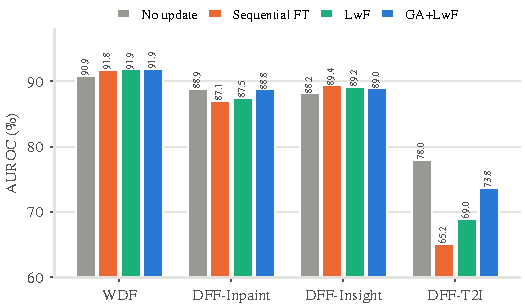
\includegraphics[width=\columnwidth]{figures/fig_unseen_breakdown.pdf}
\caption{Sealed unseen datasets after all updates on stream S1. Most of the generalization lost by updating concerns fully synthetic faces (DFF text-to-image), where GA+LwF retains 73.8 AUROC against 65.2 for sequential fine-tuning.}
\label{fig:unseen}
\end{figure}

\begin{figure}[t]
\centering
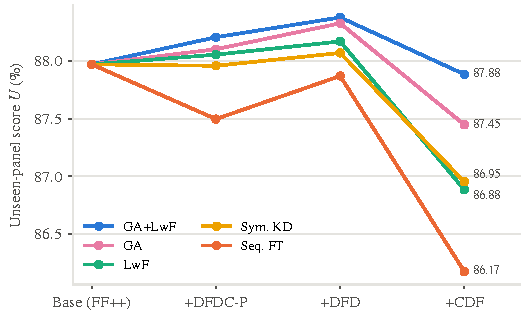
\includegraphics[width=\columnwidth]{figures/fig_stagewise.pdf}
\caption{Unseen-panel score of intermediate models along stream S1. Most of the generalization is lost at the final Celeb-DF update.}
\label{fig:stagewise}
\end{figure}

\begin{figure}[t]
\centering
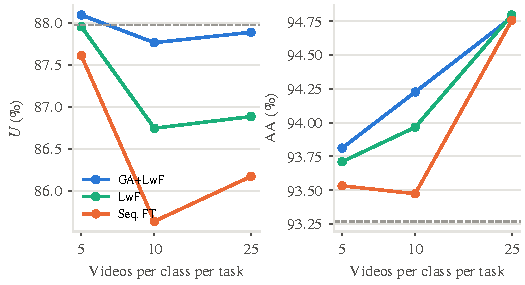
\includegraphics[width=\columnwidth]{figures/fig_shots.pdf}
\caption{Unseen-panel score (left) and mean test AUROC on the trained datasets (right) as a function of the number of videos per class and task. Dashed lines mark the never-updated detector.}
\label{fig:shots}
\end{figure}

\section{Representation analyses}
Fig.~\ref{fig:drift} relates genuine-feature drift to the change in the unseen score over 22 runs, Fig.~\ref{fig:driftmaps} localizes the drift on the grid of patch tokens, the t-SNE embeddings of the probe features are in Fig.~\ref{M-fig:tsne} of the main paper, and Fig.~\ref{fig:examples} shows unseen faces lost by sequential fine-tuning and those missed by GA+LwF.

\begin{figure}[t]
\centering
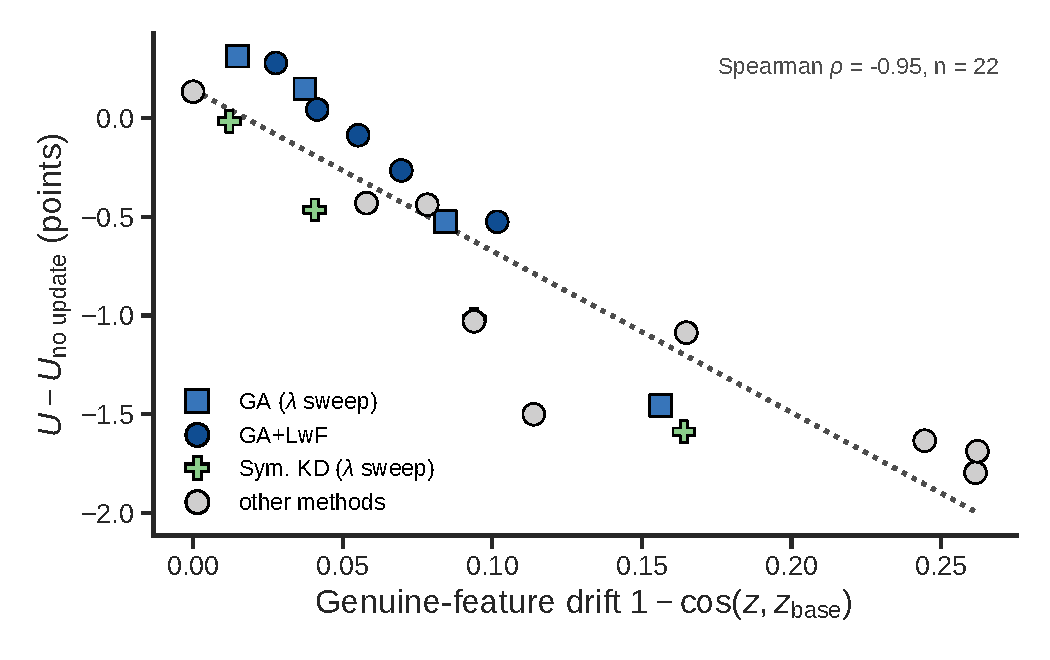
\includegraphics[width=\columnwidth]{figures/fig_drift.pdf}
\caption{Genuine-feature drift of the final model with respect to the initial model versus the change in unseen-panel score, for 22 runs on stream S1 (all methods and weight sweeps).}
\label{fig:drift}
\end{figure}

\begin{figure}[t]
\centering
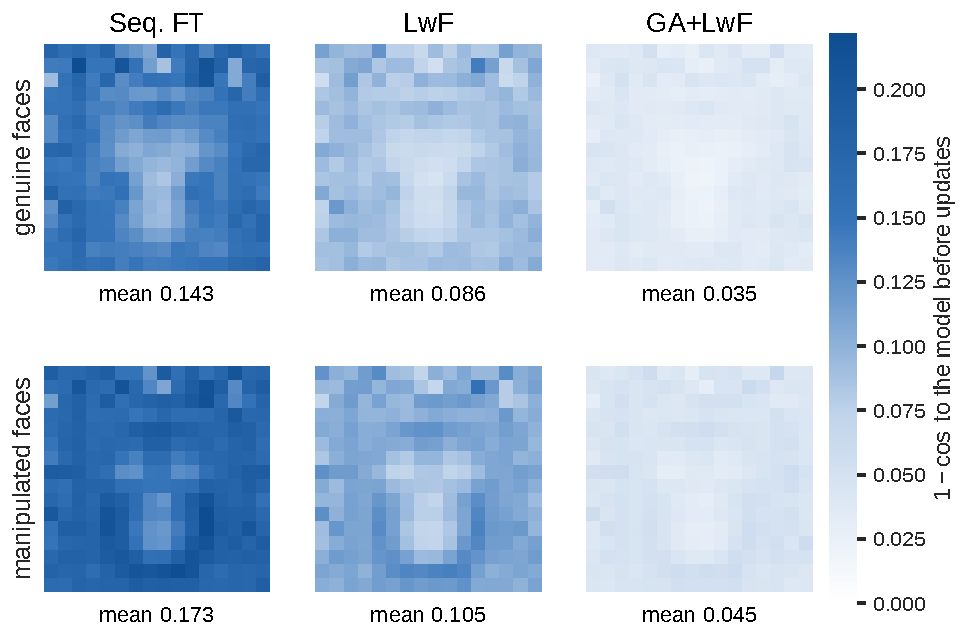
\includegraphics[width=\columnwidth]{figures/fig_driftmaps.pdf}
\caption{Mean drift of last-layer patch tokens with respect to the model before updates, over the probe set of genuine faces (top) and manipulated faces (bottom). Lighter is more stable.}
\label{fig:driftmaps}
\end{figure}

\begin{figure*}[t]
\centering
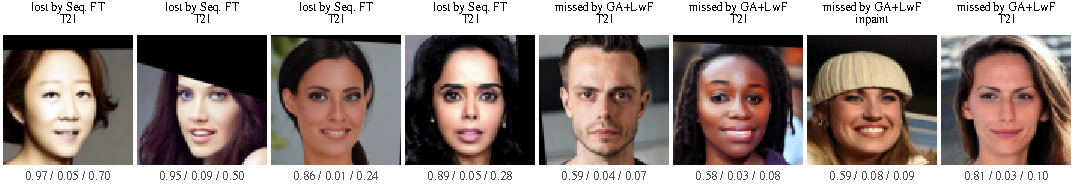
\includegraphics[width=\textwidth]{figures/fig_examples.pdf}
\caption{Unseen DeepFakeFace faces with the largest loss under sequential fine-tuning (left four) and the manipulated faces that GA+LwF misses with the lowest score among those detected by the original model (right four). Numbers: fake probability before updates, after Seq.\ FT and after GA+LwF.}
\label{fig:examples}
\end{figure*}

\section{Registered hypotheses, per-manipulation results, robustness and sensitivity}
Table~\ref{tab:hyp} lists the hypotheses of the confirmation and first extension stages with their intervals and Holm-adjusted $p$-values. Table~\ref{tab:permanip} breaks the trained datasets down by manipulation method. Fig.~\ref{fig:seeds} shows the unseen score of the five training seeds, Fig.~\ref{fig:lambda} the sensitivity to the alignment and distillation weights, and Fig.~\ref{fig:robust} the unseen score under image degradations.

\begin{table}[t]
\caption{Pre-registered hypotheses on the unseen-panel score $U$. A hypothesis is confirmed if $\Delta U>0$ and its paired bootstrap 95\% interval excludes zero. $p_{\mathrm{H}}$: Holm-adjusted one-sided $p$-value over all 18 tests (10{,}000 resamples; the smallest attainable value is 0.0018). C1: confirmation stage; M: mechanism controls; R: replication.}
\label{tab:hyp}
\centering
\footnotesize
\setlength{\tabcolsep}{2.4pt}
\resizebox{\columnwidth}{!}{%
\begin{tabular}{@{}llccc@{}}
\toprule
Hypothesis & Setting & $\Delta U$ & 95\% CI & $p_{\mathrm{H}}$ \\
\midrule
C1 GA+LwF $>$ LwF & S1 & +1.00 & [+0.70, +1.28] & 0.002 \\
C1 GA+LwF $>$ Seq.\ FT & S1 & +1.71 & [+1.01, +2.42] & 0.002 \\
C1 GA $>$ Sym.\ KD & S1 & +0.49 & [+0.31, +0.69] & 0.014 \\
\midrule
M1 GA $>$ random-subset KD & S1 & +0.51 & [+0.33, +0.70] & 0.002 \\
M2 GA $>$ fake-only KD & S1 & +0.98 & [+0.66, +1.35] & 0.002 \\
M3 GA+LwF $>$ Sym.\ KD+LwF & S1 & +0.34 & [+0.23, +0.47] & 0.002 \\
\midrule
R1 GA+LwF $>$ LwF & S2 & +0.80 & [+0.47, +1.15] & 0.002 \\
 & S3 & +1.14 & [+0.84, +1.49] & 0.002 \\
 & PE & +2.39 & [+1.57, +3.32] & 0.002 \\
R2 GA+LwF $>$ Seq.\ FT & S2 & +0.69 & [+0.06, +1.35] & 0.014 \\
 & S3 & +1.82 & [+1.13, +2.48] & 0.002 \\
 & PE & +2.13 & [+1.07, +3.20] & 0.002 \\
R3 GA $>$ Sym.\ KD & S2 & +0.37 & [+0.18, +0.56] & 0.002 \\
 & S3 & +0.54 & [+0.33, +0.76] & 0.002 \\
 & PE & +0.78 & [+0.44, +1.12] & 0.002 \\
R4 GA+LwF $>$ Sym.\ KD+LwF & S2 & +0.34 & [+0.23, +0.47] & 0.002 \\
 & S3 & +0.44 & [+0.31, +0.59] & 0.002 \\
 & PE & +0.58 & [+0.30, +0.87] & 0.002 \\
\bottomrule
\end{tabular}%
}
\end{table}

\begin{figure}[t]
\centering
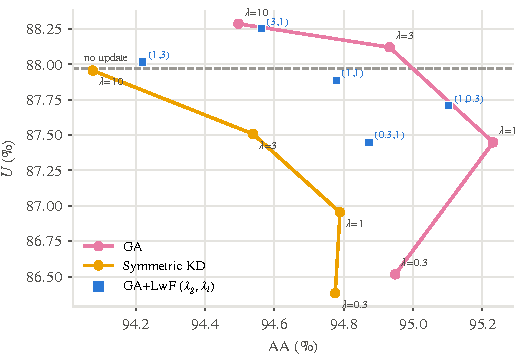
\includegraphics[width=\columnwidth]{figures/fig_lambda.pdf}
\caption{Sensitivity to the distillation weight on stream S1. Each line traces one family over $\lambda\in\{0.3,1,3,10\}$; squares show GA+LwF with weights $(\lambda_g,\lambda_l)$. The genuine-anchored frontier dominates the symmetric one at every weight.}
\label{fig:lambda}
\end{figure}



\section{Label-independent face selection}
Table~\ref{tab:labelindep} compares mask-based and largest-face crops (Section~\ref{M-sec:labelindep} of the main paper).

\begin{table}[t]
\caption{Test AUROC (8 frames per video) of the final S1 models with mask-based crops of manipulated videos (mask) and with largest-face crops for every video (largest). AA: mean over the four trained datasets (DFDC-P and Celeb-DF involve no masks).}
\label{tab:labelindep}
\centering
\footnotesize
\setlength{\tabcolsep}{2.6pt}
\begin{tabular}{@{}lcccccc@{}}
\toprule
& \multicolumn{2}{c}{\ffpp{}} & \multicolumn{2}{c}{DFD} & \multicolumn{2}{c}{AA} \\
\cmidrule(lr){2-3}\cmidrule(lr){4-5}\cmidrule(lr){6-7}
Method & mask & largest & mask & largest & mask & largest \\
\midrule
No update & 98.06 & 97.85 & 97.38 & 90.82 & 93.27 & 91.58 \\
Seq.\ FT & 96.69 & 96.56 & 96.64 & 91.60 & 94.76 & 93.47 \\
LwF & 97.98 & 97.76 & 97.18 & 92.03 & 94.80 & 93.46 \\
Sym.\ KD+LwF & 98.26 & 98.11 & 97.69 & 92.50 & 94.56 & 93.23 \\
GPL$^\dagger$ & 95.99 & 95.78 & 95.26 & 90.72 & 94.78 & 93.59 \\
GA & 98.09 & 97.95 & 97.99 & 92.66 & 95.23 & 93.86 \\
GA+LwF & 98.32 & 98.15 & 98.15 & 92.50 & 94.78 & 93.32 \\
\bottomrule
\end{tabular}
\end{table}

\section{Replication and calibration}
Fig.~\ref{fig:replication} shows the unseen score of the main methods in the four replication settings and Table~\ref{tab:calib} the 32-frame evaluation and calibration of the final S1 models (Sections~\ref{M-sec:results} and \ref{M-sec:calib} of the main paper).

\begin{table}[t]
\caption{32-frame evaluation and calibration of final models on stream S1. AA$_{32}$: mean test AUROC with 32 frames; ECE: expected calibration error (15 bins) on test splits and on the unseen panel; FPR: mean false-positive rate on genuine test videos at threshold 0.5.}
\label{tab:calib}
\centering
\footnotesize
\setlength{\tabcolsep}{3.5pt}
\begin{tabular}{@{}lcccc@{}}
\toprule
Method & AA$_{32}$ & ECE (test) & ECE (panel) & FPR (\%) \\
\midrule
No update & 93.33 & 0.056 & 0.061 & 22.1 \\
Head-only FT & 93.35 & 0.063 & 0.056 & 16.9 \\
Seq.\ FT & 95.06 & 0.040 & 0.118 & 4.3 \\
EWC & 95.06 & 0.041 & 0.113 & 3.7 \\
Replay & 95.06 & 0.040 & 0.124 & 3.5 \\
LwF & 94.97 & 0.056 & 0.090 & 5.5 \\
Symmetric KD & 95.04 & 0.044 & 0.100 & 5.3 \\
Symmetric KD + LwF & 94.71 & 0.066 & 0.081 & 8.6 \\
GA & 95.44 & 0.050 & 0.113 & 6.3 \\
GA+LwF & 94.85 & 0.072 & 0.081 & 9.7 \\
\bottomrule
\end{tabular}
\end{table}

\section{Additional figures and tables for the main results}
The following figures and tables complement Sections V-B and V-C of the main paper: the per-manipulation results, the replication across task orders and backbones, the five training seeds and the robustness to image degradations.

\begin{figure}[t]
\centering
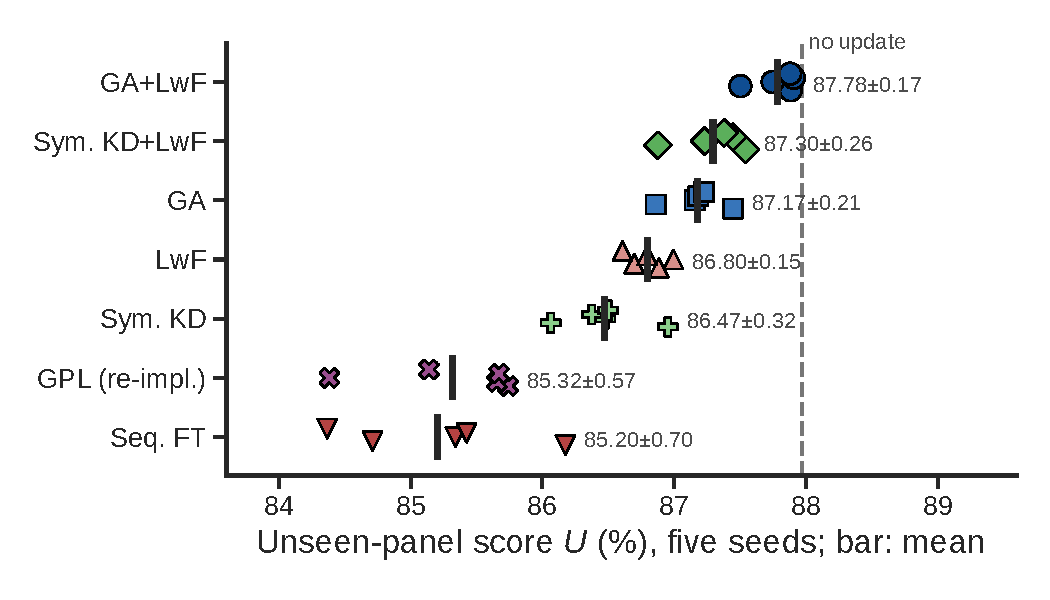
\includegraphics[width=\columnwidth]{figures/fig_seeds.pdf}
\caption{Unseen-panel score of the final S1 models for five training seeds (dots) and their mean (bar). The dashed line is the never-updated detector.}
\label{fig:seeds}
\end{figure}

\begin{figure*}[t]
\centering
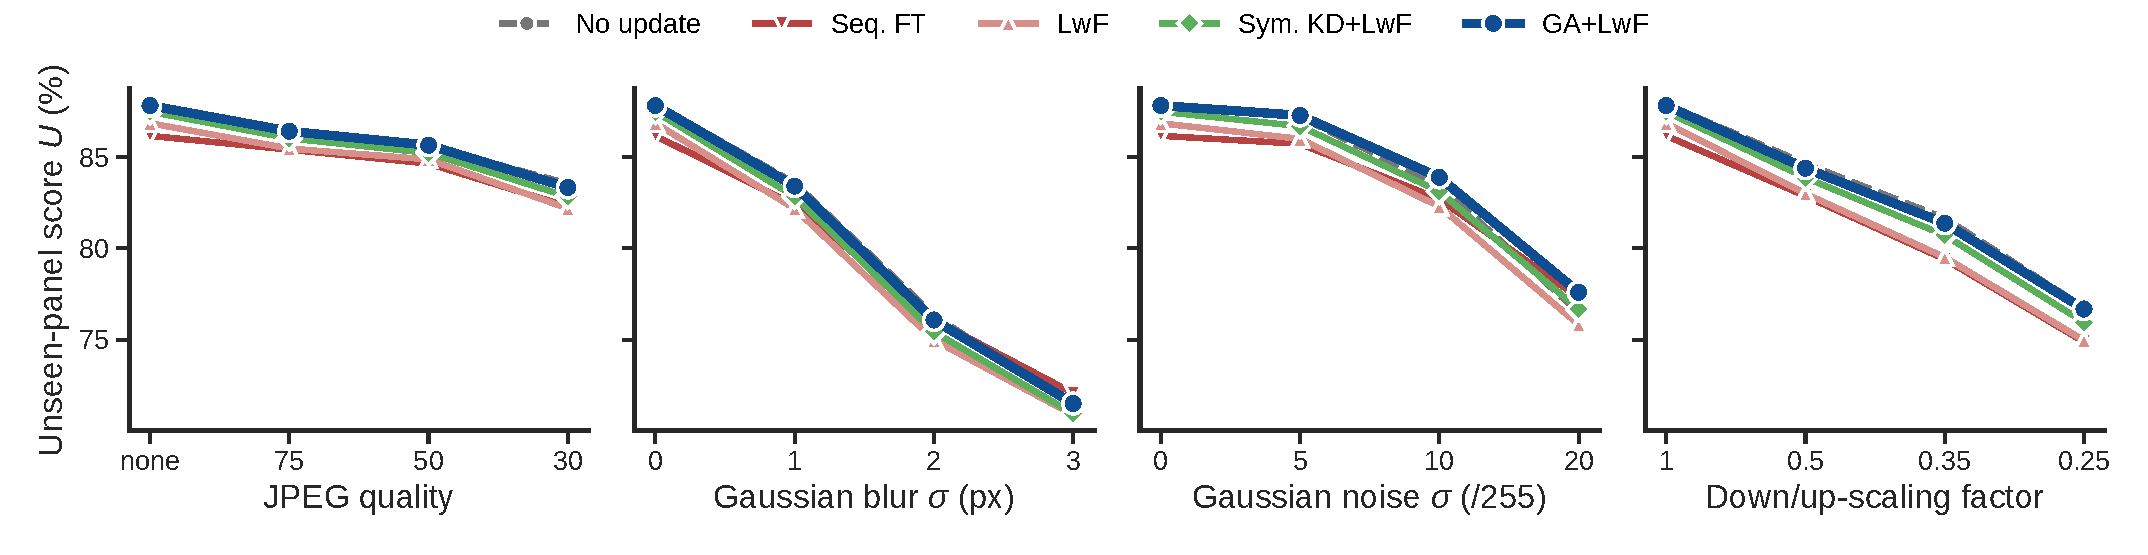
\includegraphics[width=\textwidth]{figures/fig_robust.pdf}
\caption{Unseen-panel score of the final S1 models under JPEG compression, Gaussian blur, Gaussian noise and down/up-scaling of increasing severity (WildDeepfake with eight frames per sequence). The dashed line is the never-updated detector.}
\label{fig:robust}
\end{figure*}

\begin{table}[t]
\caption{Per-manipulation test AUROC after all updates on stream S1 (32 frames per video). Each column compares the genuine test videos of the dataset with one manipulation method. FSh: FaceShifter probe (\ffpp{} development identities, never trained; 8 frames per video).}
\label{tab:permanip}
\centering
\footnotesize
\setlength{\tabcolsep}{2.7pt}
\begin{tabular}{@{}lccccccc@{}}
\toprule
& \multicolumn{4}{c}{\ffpp{} (base task)} & \multicolumn{2}{c}{DFDC-P} & \\
\cmidrule(lr){2-5}\cmidrule(lr){6-7}
Method & DF & F2F & FS & NT & A & B & FSh \\
\midrule
No update & 99.41 & 98.54 & 98.91 & 95.98 & 85.66 & 85.70 & 83.70 \\
Head-only FT & 99.37 & 98.55 & 98.97 & 95.83 & 85.20 & 85.75 & 83.67 \\
Seq.\ FT & 99.55 & 98.53 & 99.76 & 90.79 & 90.92 & 92.01 & 78.34 \\
EWC & 99.54 & 98.45 & 99.73 & 90.59 & 90.70 & 93.12 & 77.63 \\
Replay & 99.51 & 98.42 & 99.77 & 91.08 & 89.65 & 93.83 & 79.76 \\
LwF & 99.54 & 98.90 & 99.50 & 95.03 & 89.61 & 88.81 & 80.93 \\
Symmetric KD & 99.49 & 98.94 & 99.55 & 94.64 & 89.14 & 88.13 & 80.31 \\
Sym.\ KD + LwF & 99.48 & 98.86 & 99.34 & 95.82 & 88.04 & 87.12 & 82.72 \\
GA & 99.48 & 98.87 & 99.58 & 95.27 & 89.54 & 88.31 & 81.80 \\
GA+LwF & 99.47 & 98.86 & 99.41 & 95.88 & 88.19 & 87.29 & 83.19 \\
\bottomrule
\end{tabular}
\end{table}

\begin{figure*}[t]
\centering
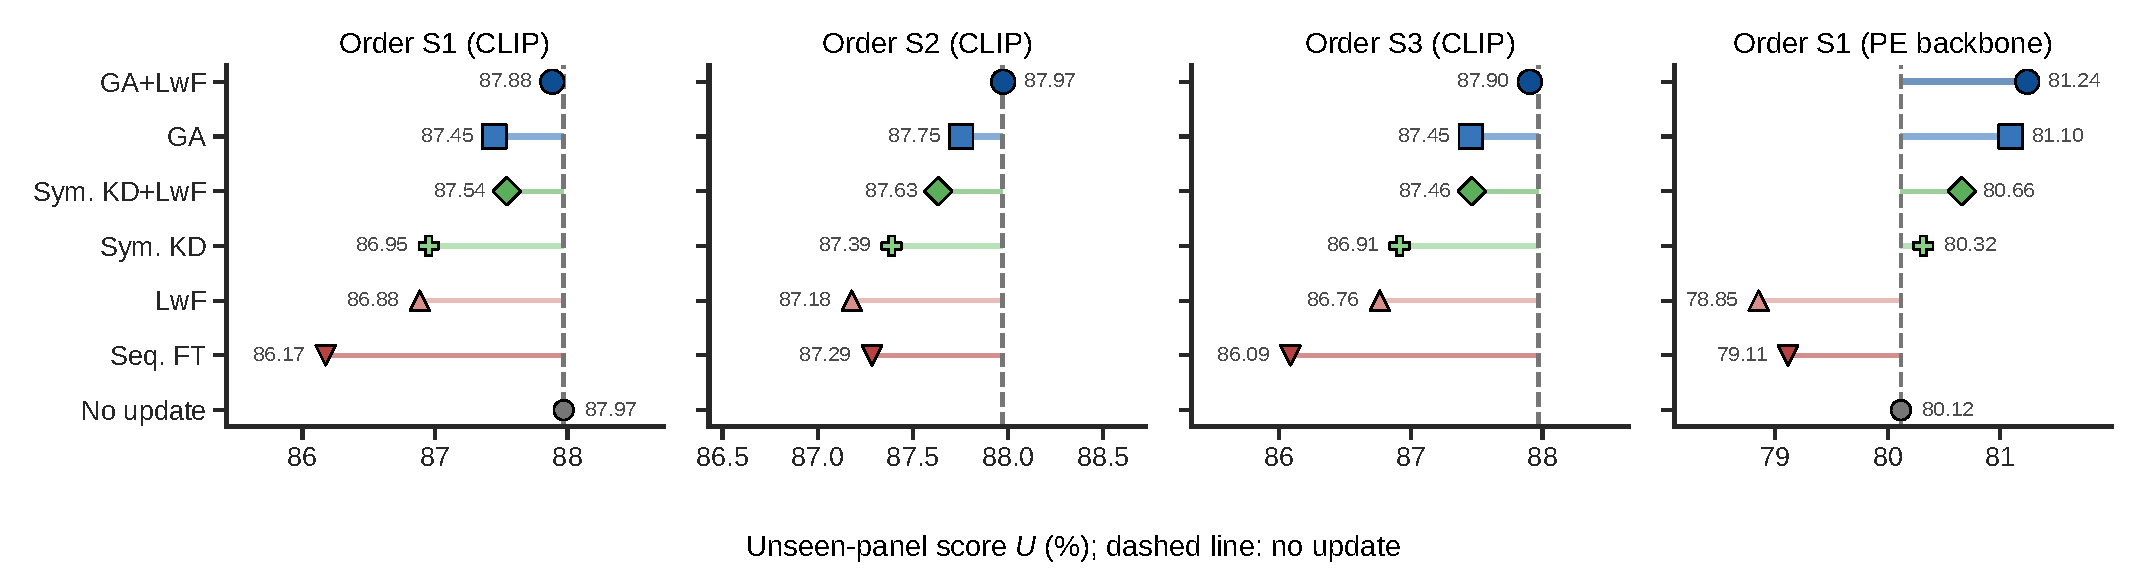
\includegraphics[width=\textwidth]{figures/fig_replication.pdf}
\caption{Unseen-panel score after all updates for the main methods in four settings: three task orders with the clean retrained CLIP-based GenD and order S1 with the released Perception Encoder variant. The dashed line marks the never-updated detector of each setting.}
\label{fig:replication}
\end{figure*}

\section{Weight selection, reproduction of GenD and misranked pairs}
Algorithm~\ref{alg:select} gives the development-data procedure for choosing the alignment weight (Section V-C of the main paper), Table~\ref{tab:repro} compares reported and reproduced GenD scores, and Fig.~\ref{fig:margin} shows the fraction of genuine and manipulated pairs that are misranked by the updates as a function of their margin before the updates.

\begin{algorithm}[t]
\caption{Development-selected alignment weight}
\label{alg:select}
\footnotesize
\begin{algorithmic}[1]
\Require candidate weights $\Lambda$, target plasticity $G^{*}$ (mean gain), development splits
\For{each $\lambda\in\Lambda$}
  \State run Algorithm~\ref{M-alg:stream} on the development splits with $\lambda_g=\lambda$
  \State $G(\lambda)\gets$ mean gain of the run
\EndFor
\State $\lambda^{*}\gets\arg\min_{\lambda\in\Lambda}|G(\lambda)-G^{*}|$ \Comment{ties: larger $\lambda$}
\State \Return $\lambda^{*}$ \Comment{sealed test data and panel never used}
\end{algorithmic}
\end{algorithm}

\begin{table}[t]
\caption{Video AUROC (\%) of GenD. Released weights are evaluated with our pipeline; the retrained model selects its checkpoint on \ffpp{} validation only. Dashes denote values that were not reported or not evaluated.}
\label{tab:repro}
\centering
\footnotesize
\setlength{\tabcolsep}{4pt}
\begin{tabular}{@{}lccc@{}}
\toprule
Test set & Paper~\cite{yermakov2026gend} & Released weights & Clean retrain \\
\midrule
\ffpp{} test & \textendash & \textendash & 98.21 \\
Celeb-DF v2 & 94.6 & 95.11 [92.95, 96.81] & 92.04 \\
DFD & 96.4 & 97.59 [96.80, 98.30] & \textendash \\
DFDC-P & \textendash & 90.00 & 85.66 \\
\bottomrule
\end{tabular}
\end{table}

\begin{figure}[t]
\centering
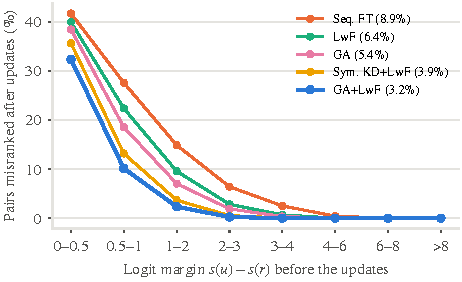
\includegraphics[width=\columnwidth]{figures/fig_margin.pdf}
\caption{Fraction of correctly ranked genuine and manipulated pairs of the unseen panel that are misranked after the S1 updates, by logit margin before the updates (post hoc). Legend: overall fraction.}
\label{fig:margin}
\end{figure}

\section{Recalibration with current-task data}
Table~\ref{tab:recal} reports the recalibration study discussed in Section~\ref{M-sec:calib} of the main paper.

\begin{table}[t]
\caption{Recalibration after the last update using only current-task data (25 genuine and 25 manipulated Celeb-DF development videos). ECE on the four test splits and on the unseen panel, without recalibration (raw), with a fitted bias and with Platt scaling; ACC: mean test accuracy at threshold 0.5 (\%).}
\label{tab:recal}
\centering
\footnotesize
\setlength{\tabcolsep}{2.4pt}
\begin{tabular}{@{}lcccccccc@{}}
\toprule
& \multicolumn{3}{c}{ECE, test} & \multicolumn{3}{c}{ECE, unseen panel} & \multicolumn{2}{c}{ACC, test} \\
\cmidrule(lr){2-4}\cmidrule(lr){5-7}\cmidrule(lr){8-9}
Method & raw & bias & Platt & raw & bias & Platt & raw & Platt \\
\midrule
No update & 0.056 & 0.056 & 0.049 & 0.061 & 0.080 & 0.114 & 87.8 & 83.9 \\
Seq.\ FT & 0.040 & 0.043 & 0.082 & 0.118 & 0.107 & 0.177 & 83.3 & 85.5 \\
LwF & 0.056 & 0.066 & 0.042 & 0.090 & 0.075 & 0.146 & 85.0 & 87.0 \\
Sym.\ KD+LwF & 0.066 & 0.062 & 0.058 & 0.081 & 0.083 & 0.160 & 86.9 & 86.6 \\
GA & 0.050 & 0.051 & 0.065 & 0.113 & 0.112 & 0.185 & 86.9 & 87.6 \\
GA+LwF & 0.072 & 0.066 & 0.054 & 0.081 & 0.091 & 0.167 & 87.6 & 87.0 \\
\bottomrule
\end{tabular}
\end{table}

\bibliographystyle{IEEEtran}
\bibliography{references}

\end{document}
